
\section{Experimental Results}
In this section we evaluate the efficiency of SBS.
First, we exhibit the benefits of striping the data by monitoring the patterns captured at different time scales.
Second, we thoroughly investigate the alarms reported by SBS with the two datasets.


\begin{figure*}[t!]
% \subfloat[Raw signals]{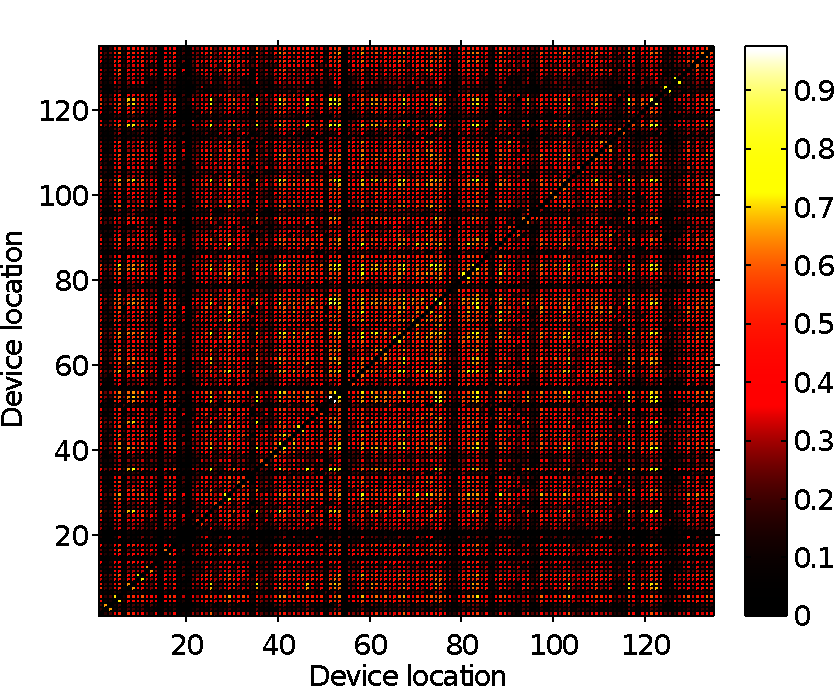
\includegraphics[width=.48\textwidth]{img/heatMap_raw_201106-eps-converted-to.pdf}}\\
\subfloat[High Frequencies\label{fig:heatmap:high}]{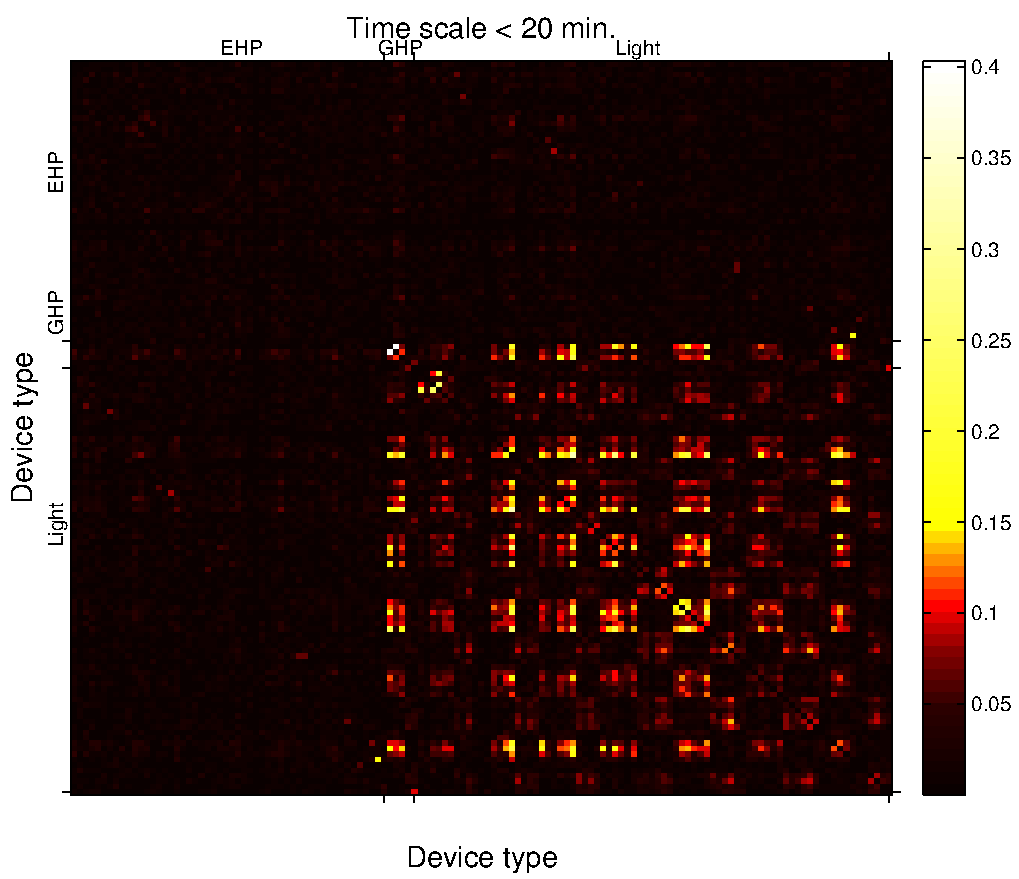
\includegraphics[width=.48\textwidth]{img/heatMap_1_201106-eps-converted-to.pdf}}\hfill
\subfloat[Medium Frequencies\label{fig:heatmap:med}]{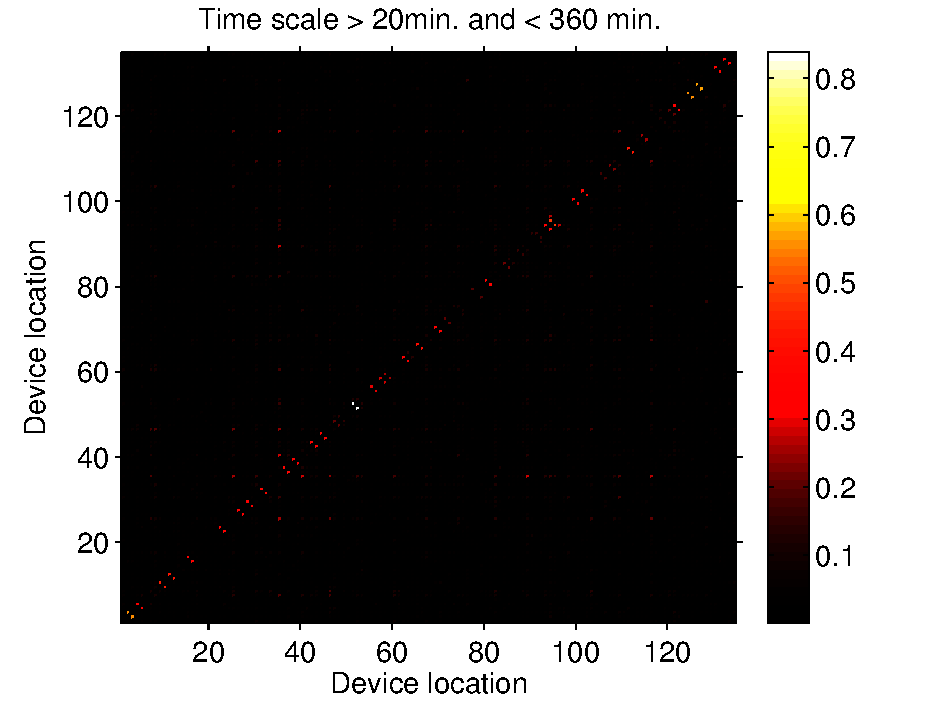
\includegraphics[width=.48\textwidth]{img/heatMap_2_201106-eps-converted-to.pdf}}\\
\subfloat[Low Frequencies\label{fig:heatmap:low}]{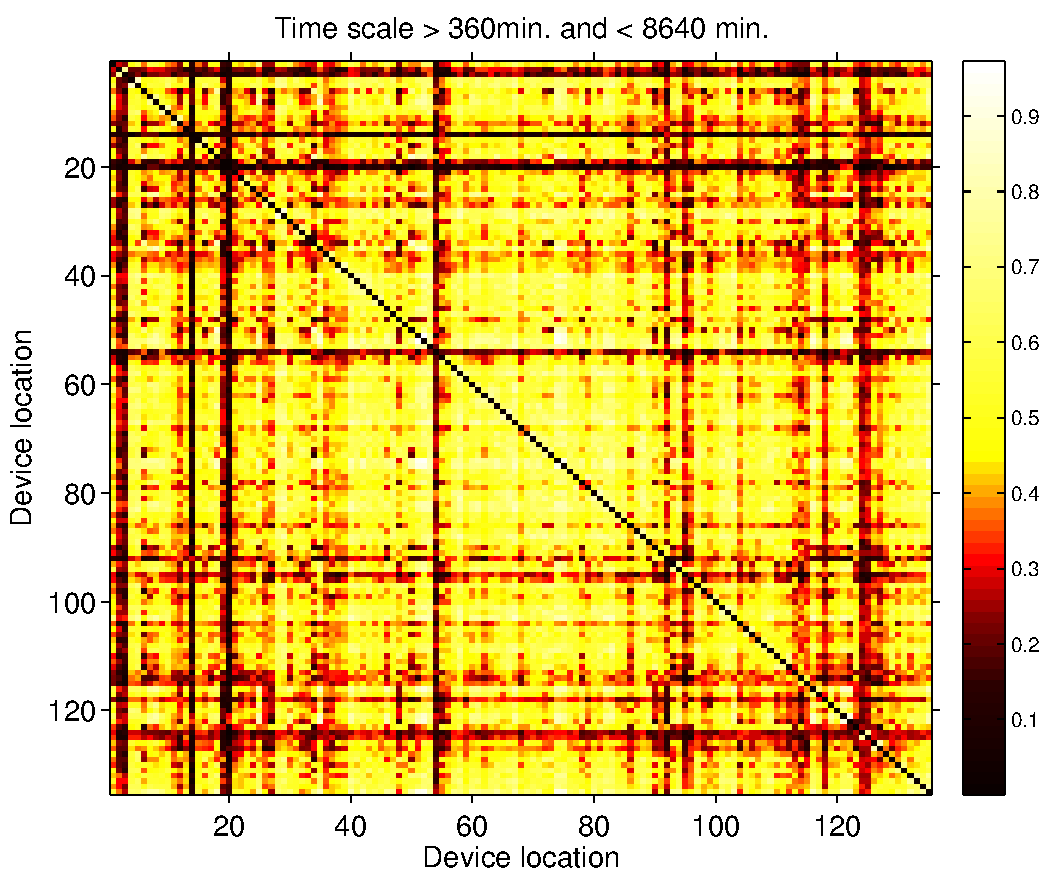
\includegraphics[width=.48\textwidth]{img/heatMap_3_201106-eps-converted-to.pdf}}\hfill
\subfloat[Residual data\label{fig:heatmap:res}]{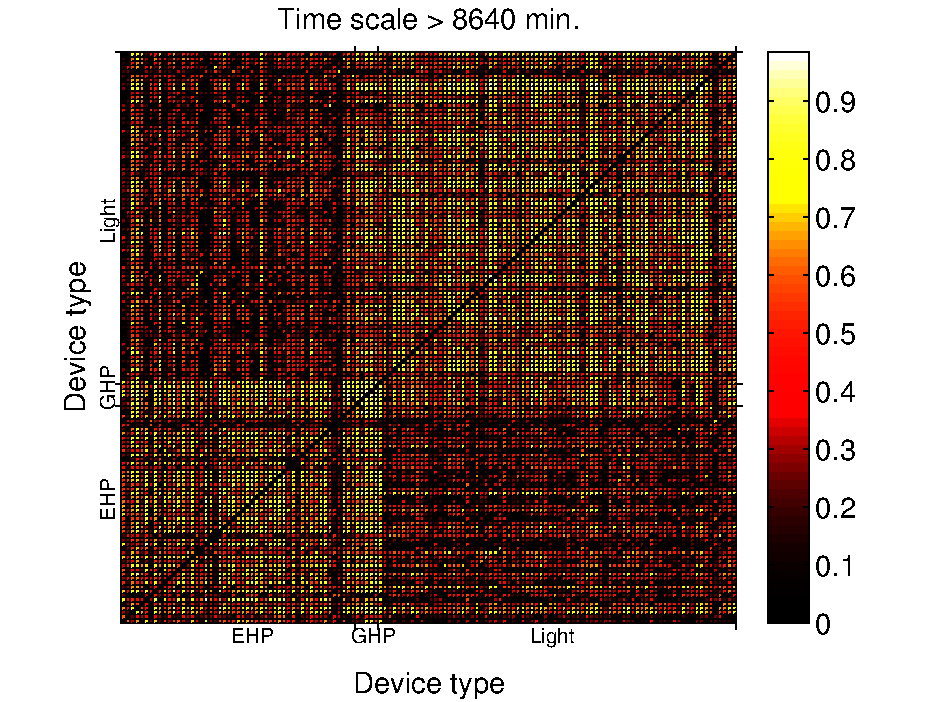
\includegraphics[width=.48\textwidth]{img/heatMap_4_201106-eps-converted-to.pdf}}
\caption{Reference correlation matrices for the four time scale ranges (the diagonal $x=y$ is colored in black for better reading). High correlation at the medium frequencies highlight devices that are located next to each other thus intrinsically related. Data at the low frequencies highlights the common daily pattern of the data. Unexpectedly the residual data permits to cluster devices of the similar type.}
\label{fig:heatmap}
\end{figure*}

\subsection{Device behavior at different time scales}
The Strip and Bind part of SBS is evaluated using the data from the Engineering Building 2 as ground truth data.
This dataset is appropriate to measure the SBS performance as we assume that the lighting and HVAC systems of the same room are intrinsically related.
Consequently, we analyze this data using SBS and verify that the higher correlations at medium frequencies correspond to devices located in the same room and the unwanted data is captured at the other frequencies.

The dataset is split in 10 bins of 1 week long, each bin being processed with SBS.
Using the 10 correlation matrices uncovered at each time scale range SBS uncovered the four reference matrices depicted in Figure \ref{fig:heatmap}.

\paragraph{High frequencies}
In this work the high frequencies correspond to the signals noise, therefore, we do not expect any beneficial information from the corresponding matrix (Fig. \ref{fig:heatmap:high}).
Indeed the corresponding reference matrix does not provide any help to discriminate devices location.
Thus, we emphasize that this data should be ignored for efficiently uncovering the devices intrinsic relationships (contrarily to \cite{romain:iotapp12}).
Interestingly, we found that the sensors monitoring the lights generate consistent noise and could help one to cluster this type of sensor.
  
\paragraph{Medium frequencies}
Our main focus is on the medium frequencies as it is designed to capture the intrinsic device relationships.
Figure \ref{fig:heatmap:med} depicts the devices correlation at the medium frequencies.
This correlation matrix is significantly different from the one of the raw signals (Fig. \ref{fig:heatmap:raw}) as higher correlation are mainly concentrated along the matrix diagonal. 
Since the devices serving the same or adjacent rooms are placed nearby in the matrix it validates our assumption; high correlation scores at the medium frequency band stand for devices intrinsic relationship.
Thus, this matrix helps us to discriminate devices that are used in concert.
For example using a community mining algorithm (i.e. the Louvain algorithm \cite{blondel:unfolding}) we identify the communities described by this reference matrix.
As expected we obtained mainly clusters of only two devices (light and HVAC serving the same room), but we also found clusters that are composed of more devices.
The biggest cluster contains 33 devices that are 2 GHP devices and the corresponding lights.
Similarly another cluster of 8 devices contains 1 GHP and the corresponding lights and the 2 other GHP are clustered together with a single light.
We also obtained a cluster containing the 3 HVAC serving the three server rooms. Although these server rooms are located at different floors SBS measured a strong correlation between these devices as they are similarly managed.
Interestingly we also observe a couple of clusters that consist of independent devices serving two adjacent rooms belonging to the same lab.
This correlation matrix and the corresponding clusters are the definite evidence of the SBS ability to uncover devices intrinsic-relationships.
 
\paragraph{Low frequencies}
Low frequencies intend to capture the daily pattern common to all the devices.
Figure \ref{fig:heatmap:low} depicts the corresponding reference matrix which is similar to the one for the raw signals (Fig. \ref{fig:heatmap:raw}) and advertises no particular structure.
Since this matrix contains mainly high values, most of the partial signals at low frequencies features similar characteristics (i.e. daily patterns).
Therefore, these partial signals are correctly discarded as they do not help us in identifying inter-device usage patterns.
 
\paragraph{Residual data}
In this experiments the residual data stands for the weekly trend of the devices.
Obviously this data provides poor insights on the devices intrinsic-relationships.
But surprisingly by reordering the correlation matrix based on the type of the devices (Figure \ref{fig:heatmap:res}) we found two major clusters.
The first cluster consists of HVAC devices (see EHP and GHP in Fig. \ref{fig:heatmap:res}) whereas the second one contains only lights. 
An in-depth examination of the data revealed that long-term trends are inherent to the device types. 
For example, as the consumption of both the EHP and GHP devices is driven by the building occupancy and the outside temperature, these two types of devices follow the same trend. 
However, the use of light is independent from the outside temperature thus the lighting systems follow a common trend that is different from the EHP and GHP one.

We conducted the same experiments by splitting the dataset in 70 bins of 1 day long and observed analogous results for short time scales but dissimilar for longer scales.
At high and medium frequencies we obtained very similar matrices, however, almost no data is captured at the low frequencies (because the bins are too short to exhibit daily oscillations) and the residual data captures only the daily trend.

% TODO add some info about the reference matrix for the Cory Hall?

\subsection{Anomalies}
We now validate the anomalies found by SBS in the traces from the Engineering Building 2 and the Cory Hall.
Nevertheless, due to the lack of ground truth data such as rooms schedule or reports of energy waste evaluating the SBS results is not straightforward.

\paragraph{Evaluation process}
To validate the SBS results we manually inspect the identified anomalies.
Therefore, for each reported alarm $(t,i)$ we thoroughly investigate the data from the device $i$ and its related devices (as provided by the reference matrix) in order to identify the root cause of the alarm.
In particular we retrieve the major relationship change that causes the alarm (i.e. $\max(|w_j(C_{i,j}^t - R_{i,j})|)$, see Section \ref{methodo:ano}) and examine the metadata associated to the corresponding device
% $j$ and the sign of the relationship change $C_{i,j}^t - R_{i,j}$.
% A positive value of relation change means the devices correlation at the time bin $t$ is abnormally high, whereas negative value means that the relationship between the two devices is broken.
This investigation allow us to classify the alarms into five groups:
\begin{itemize}
 \item \emph{High power usage}: alarms standing for electricity waste.
 \item \emph{Low power usage}: alarms caused by a device abnormal low electricity consumption.
 \item \emph{Punctual abnormal usage}: short term (less than 2.5 hours) raise or drop of the electricity consumption.
 \item \emph{Missing data}: alarms raised due to a sensor failure.
 \item \emph{Other}: alarms whose root cause is unclear.
\end{itemize}

% However, the exhaustive enumeration of the true negatives (i.e. saving opportunities that are not detected) is impractical because of the size of the analyzed datasets (number of devices and traces length).
% Instead we exhibit the detector sensitivity by varying $\tau$, the threshold value.

\begin{figure}
\begin{center}
 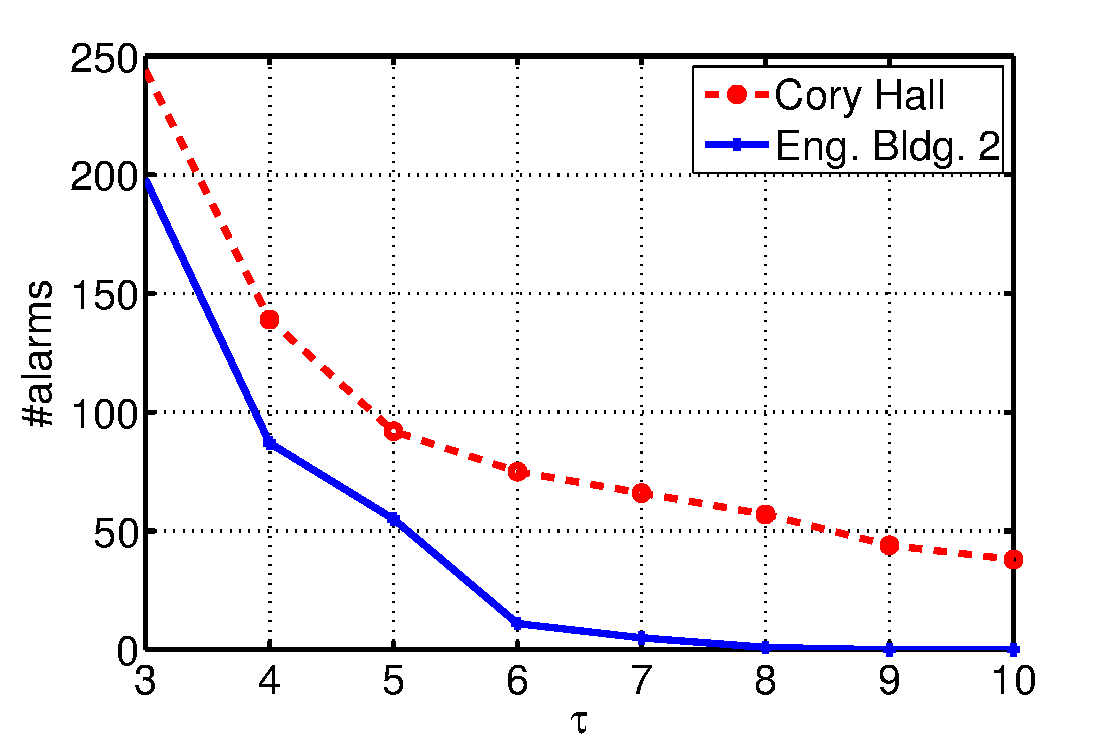
\includegraphics[width=.49\textwidth]{img/threshold-eps-converted-to.pdf}
 \caption{Number of reported alarms for various threshold value ($\tau=[3,10]$).}
 \label{fig:thres}
 \end{center}
\end{figure}

\paragraph{Experimental setup}
For all the experiments presented in this section the data is split in time bins of one day long starting from 09:00 am which is approximately the offices opening hours.
We avoid to start the time bins at midnight as we found that numerous anomalies appear at night and they are better highlighted if they are not spanning two time bins.
The reference matrix is computed using data at the medium frequencies for all the time bins.

\begin{figure*}[t]
  \subfloat[High power usage where the HVAC (EHP) is turned on at night\label{fig:res:eng1}]{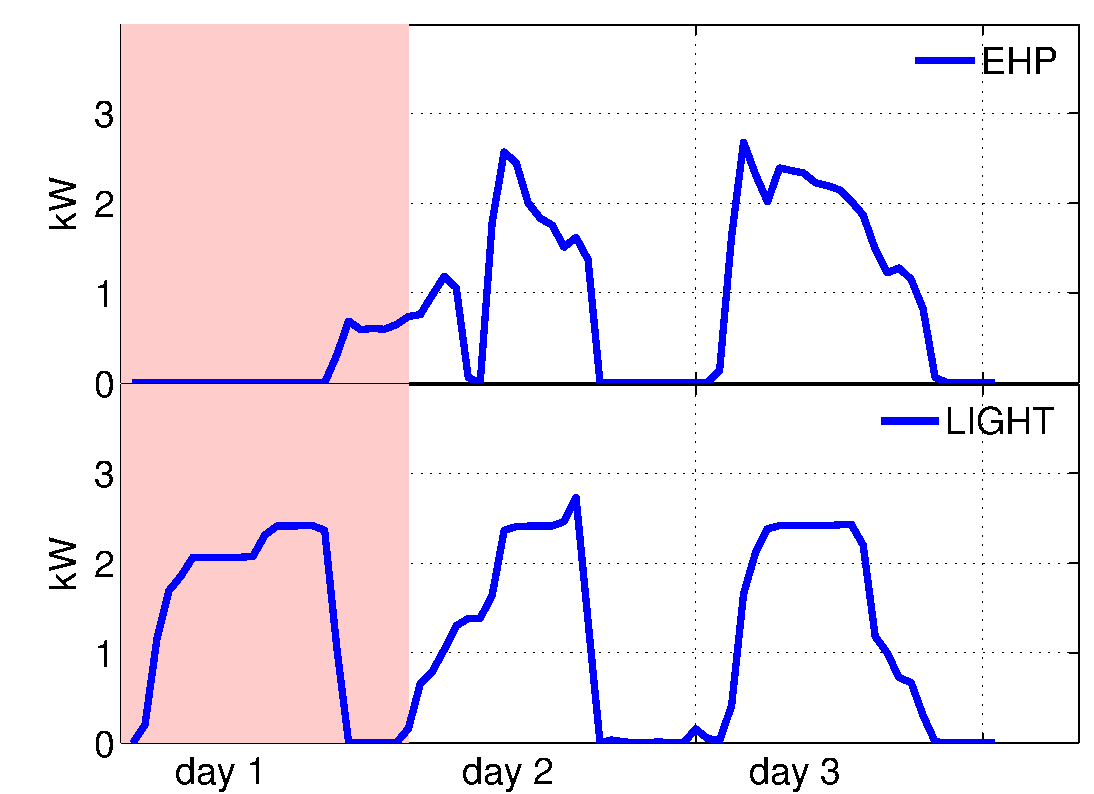
\includegraphics[width=.32\textwidth]{img/0sig20_sig31alarm1-eps-converted-to.pdf}} \hspace{.015\textwidth} %EHP turned on at night!?
  \subfloat[High power usage where the light is left on at night\label{fig:res:eng2}]{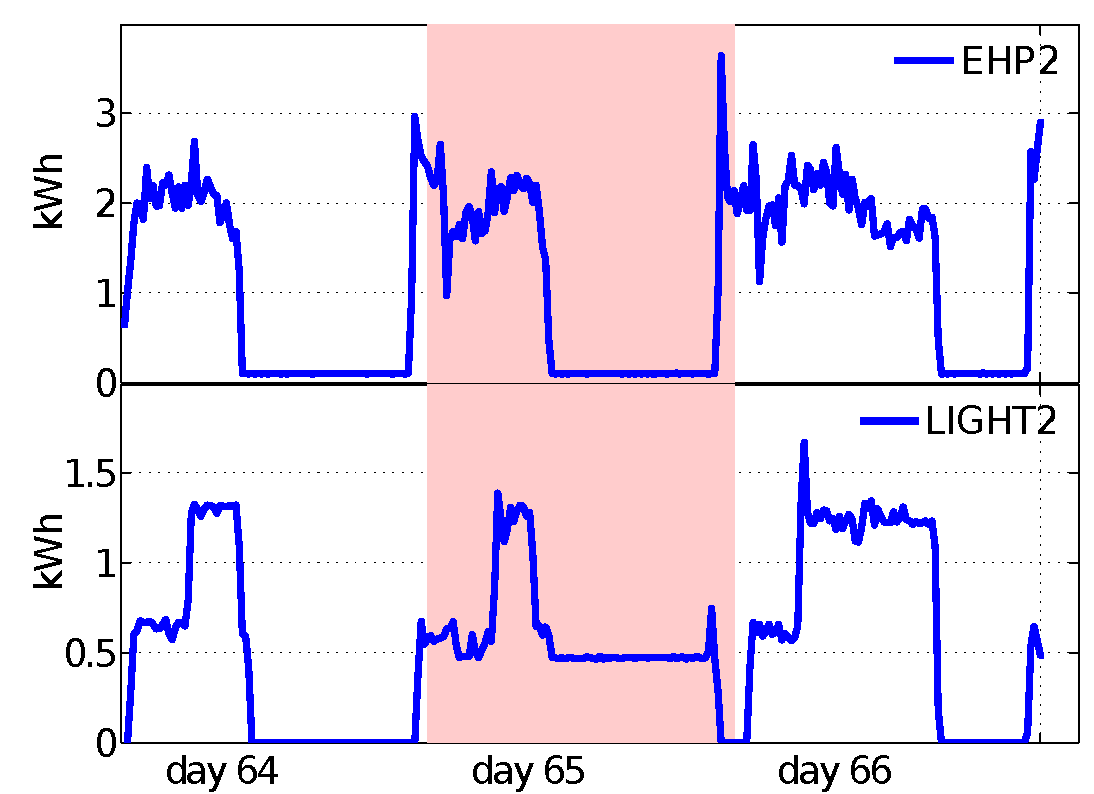
\includegraphics[width=.32\textwidth]{img/0sig123_sig134alarm65-eps-converted-to.pdf}} \hspace{.015\textwidth}  %Light left on during night
 \subfloat[Low power usage where the HVAC (EHP) is not used during office hours\label{fig:res:eng3}]{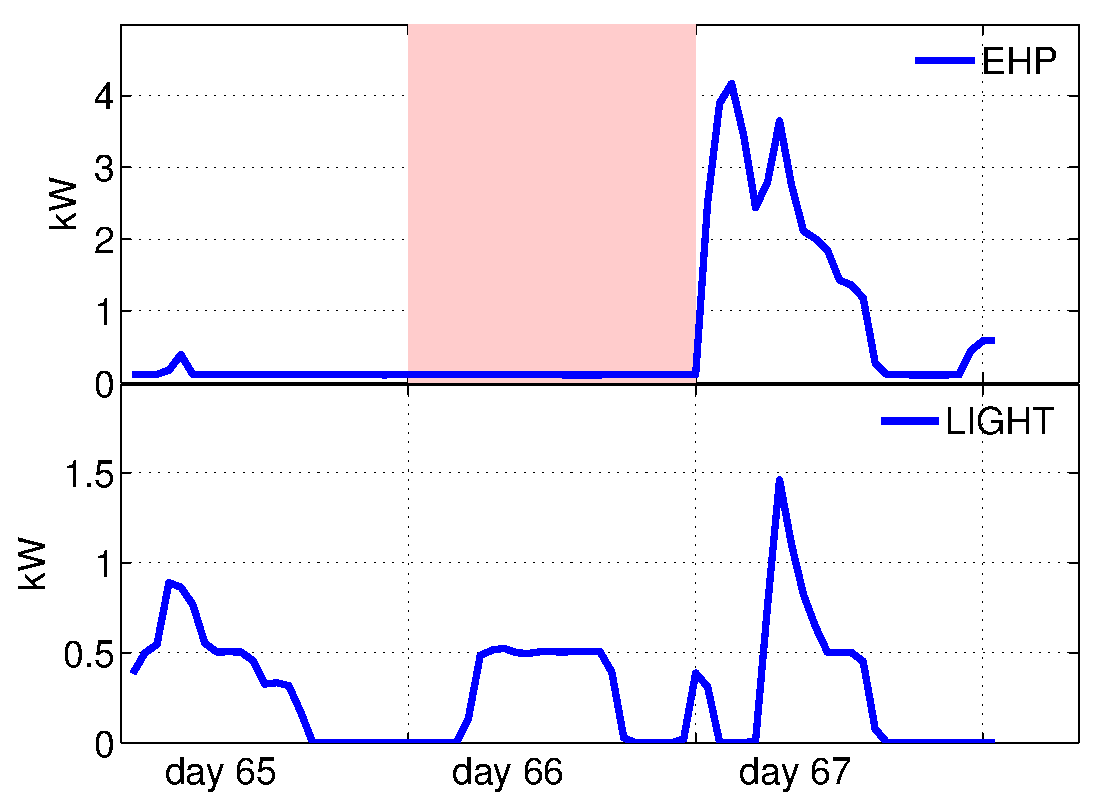
\includegraphics[width=.32\textwidth]{img/0sig24_sig33alarm66-eps-converted-to.pdf}}\\ %Three EHPs that are really correlated
 \subfloat[Long term high power usage partially detected\label{fig:res:eng4}]{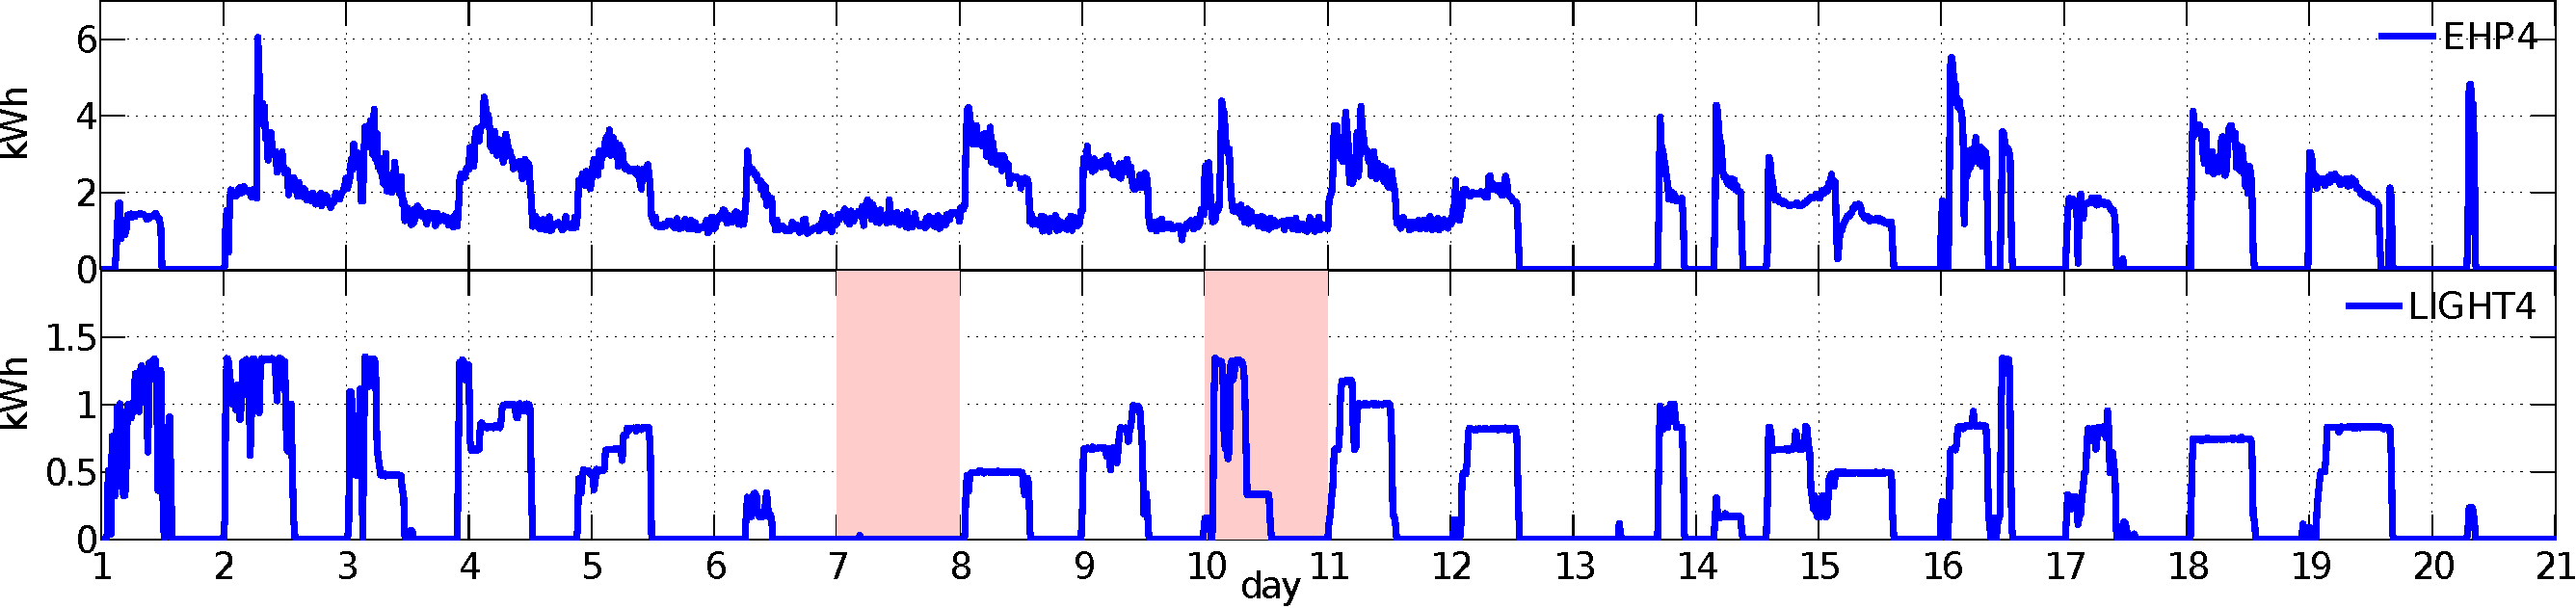
\includegraphics[width=\textwidth]{img/0sig3_sig15alarm7-eps-converted-to.pdf}}\\  
\caption{Example of alerts (red rectangles) reported by SBS using the Engineering Building 2 dataset}
\end{figure*}

By varying the threshold $\tau$ we can tune the sensitivity of SBS thus the number of reported alarms.  
Furthermore, by plotting the number of alarms against the value of $\tau$ for both datasets (Fig. \ref{fig:thres}) we observe an elbow in the graph around $\tau=5$.
With thresholds lower than this pivot value ($\tau<5$) the number of alarms is significantly increasing thus likely to report less important anomalies.
Whereas for higher value ($\tau>5$) the number of alarms is slowly decreasing thus provide a more conservative result that only consists of the most important anomalies.
As this pivot value is usually a good trade off we set $\tau=5$ for both datasets.


\subsubsection{Engineering Building 2}

\begin{table}
\begin{center}
\begin{tabular}{|l||c|c|c|c|c|}
\hline
Dataset&High&Low&Punc.&Missing&Other\\ \hline \hline
Eng. Bld. 2& 9 & 6 & 1 & 36 & 3 \\ \hline
Cory Hall& 25 & 7 & 4 & 0 & 3 \\ \hline
\end{tabular}
\end{center}
\caption{Alarms classification result for both dataset.}
\label{tab:classif}
\end{table}

SBS reported 55 alarms along the 10 weeks of the Engineering Building 2 dataset.
However, 36 alarms are discarded as they stand for missing data in the dataset; one GHP has no data for the first 18 days.
Since this device is highly correlated to another GHP in the reference matrix, their relationship is broken for the 18 first bins and two alarms per bin are raised (one for each GHP).

In spite of the post-Fukushima university measures to reduce its electricity footprint, SBS reported 9 alarms corresponding to high power usages (Table \ref{tab:classif}).
For example Figure \ref{fig:res:eng1} depicts the electricity consumption of the light and EHP of the same room for which two alarms have been raised at the first time bin.
Because the EHP was not used during daytime but has been turned on at night when the light is turned off the relationship between the two devices is broken and an alarm is raised for each device.
Figure \ref{fig:res:eng2} is another example of energy waste where the light has been left on during night whereas the EHP has been turned off.
The top-priority anomaly reported by SBS is caused by the 10 days long constant use of a room EHP (Figure \ref{fig:res:eng4}) and this waste of electricity accounts for 165 kWh.
SBS partially reported this anomaly, however, lower threshold value $\tau$ permits to identify most of it.

\begin{figure*}[t]
  \subfloat[Low power usage due to a chiller failure\label{fig:res:cory1}]{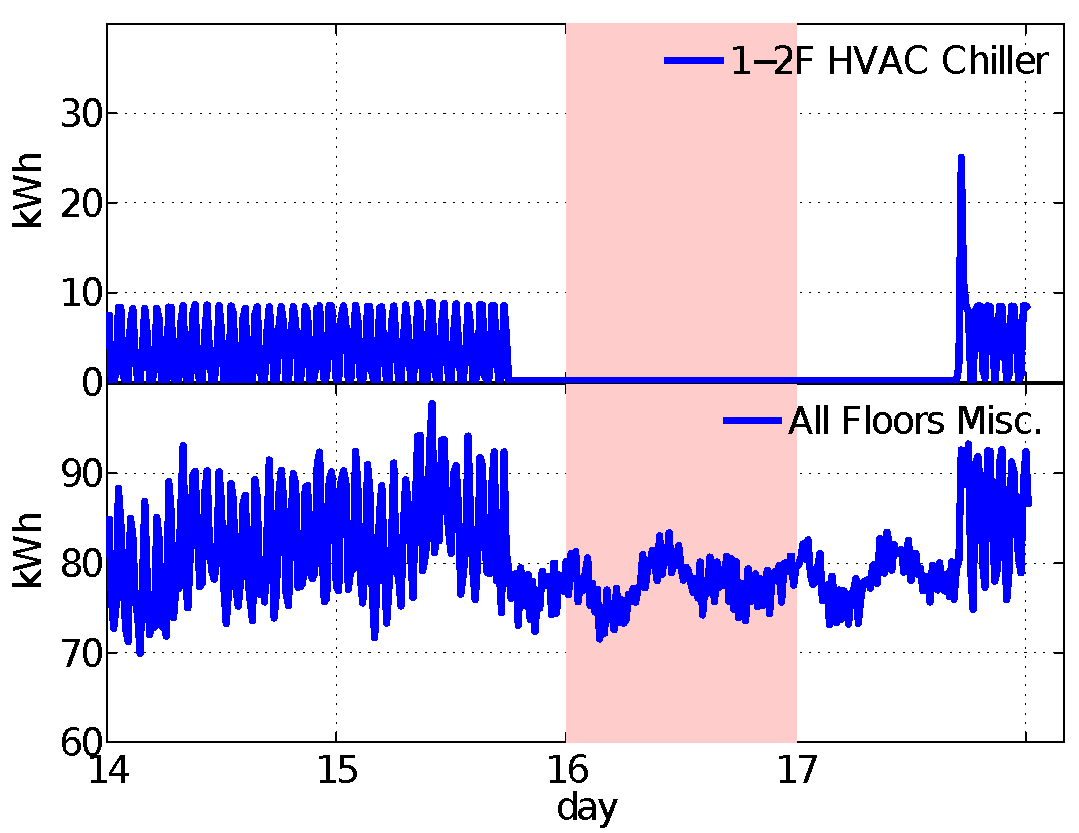
\includegraphics[width=.32\textwidth]{img/1sig37_sig55alarm16-eps-converted-to.pdf}} \hspace{.015\textwidth}
 \subfloat[High power usage highlighted by the elevator usage\label{fig:res:cory21}]{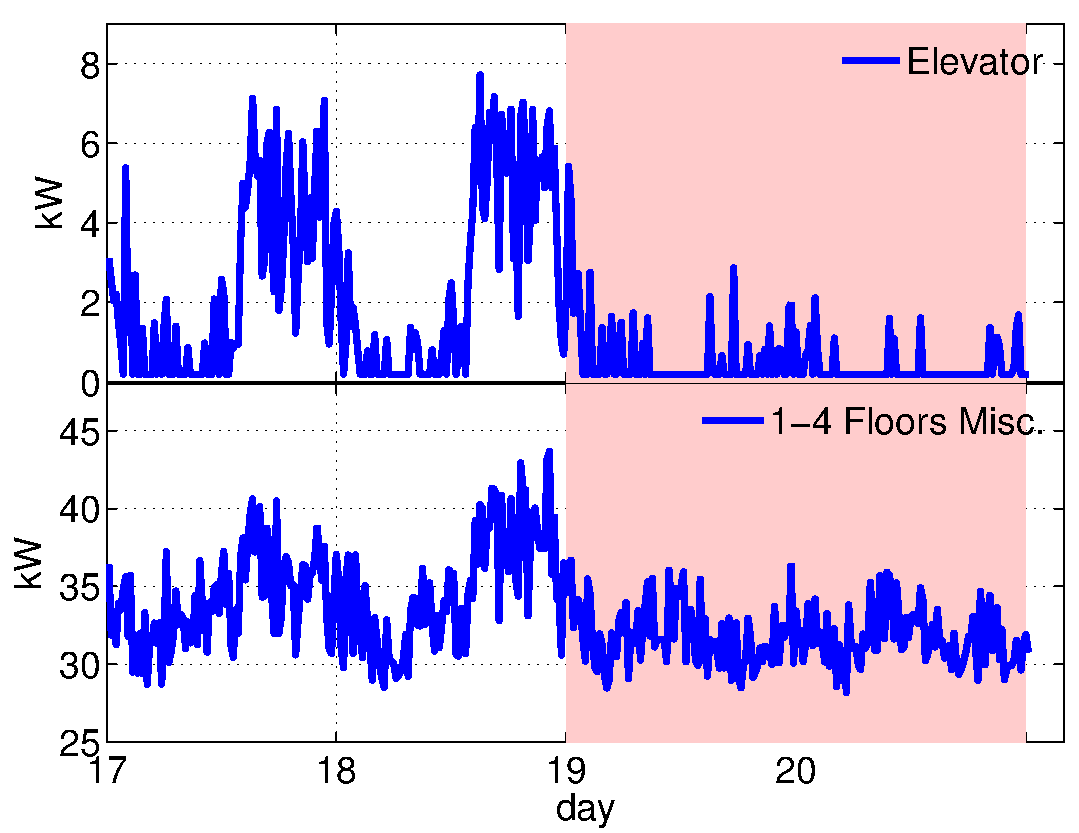
\includegraphics[width=.32\textwidth]{img/1sig7_sig49alarm19-eps-converted-to.pdf}}
 \hspace{.015\textwidth}
 \subfloat[Normal power and elevator usage\label{fig:res:cory22}]{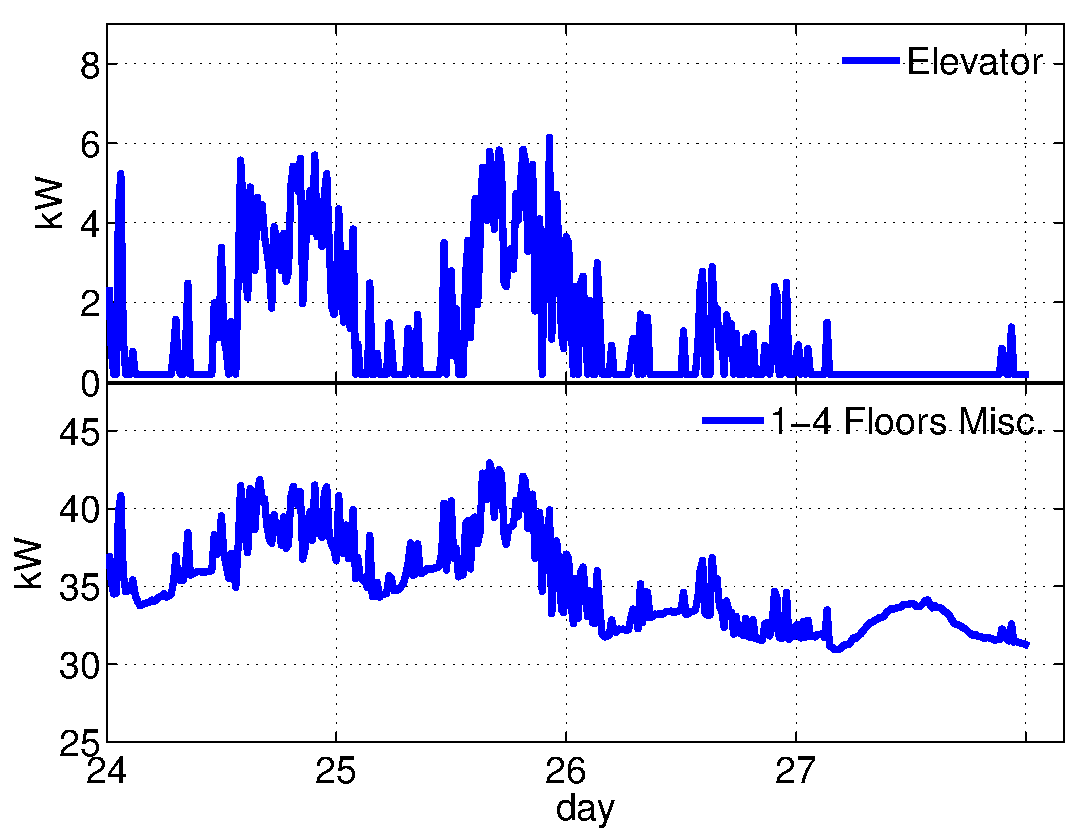
\includegraphics[width=.32\textwidth]{img/1sig7_sig49alarm-eps-converted-to.pdf}}\\ 
 \subfloat[Long term high power usage due to competing heating and cooling\label{fig:res:cory3}]{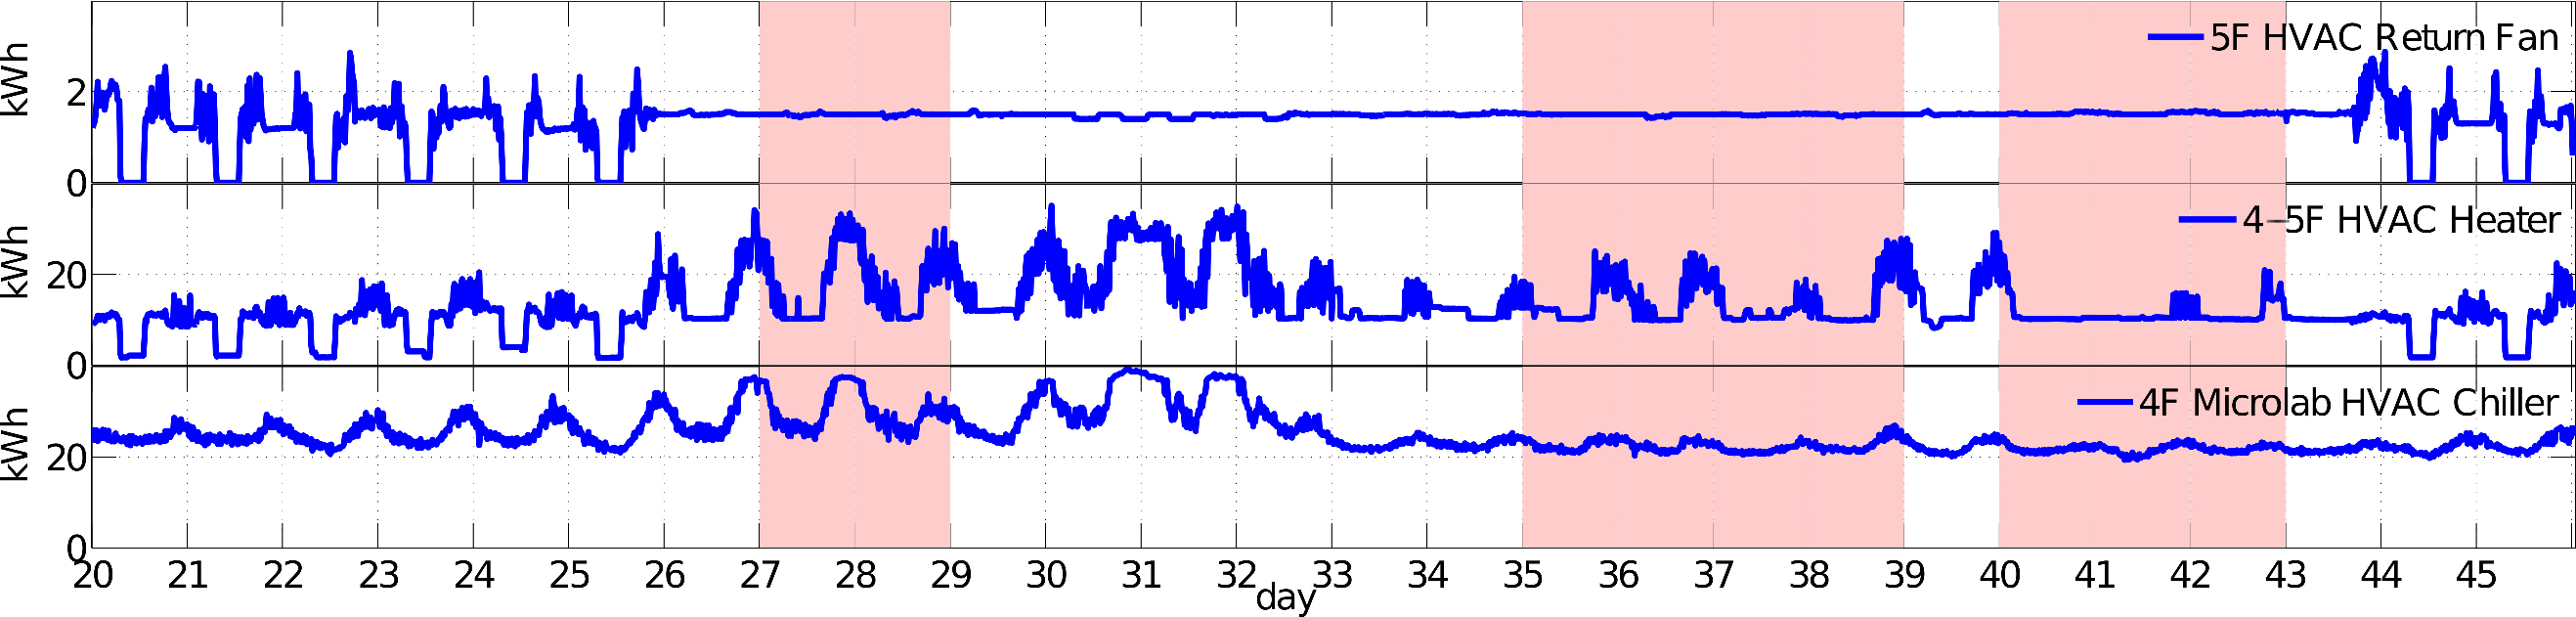
\includegraphics[width=\textwidth]{img/1sig34_sig54alarm27-eps-converted-to.pdf}} 
\caption{Example of anomalies identified by SBS for the Cory Hall dataset}
\end{figure*}

We observed 6 alarms corresponding to abnormal low power usage, our inspection revealed that they usually correspond to energy saving initiatives from the rooms users likely due to the electricity concern in Japan.
This behavior is depicted in Figure \ref{fig:res:eng3}, the occupancy is obvious as the light is used at the usual office hours but the EHP has not been turned on during daytime in the sole intention to save electricity.

\subsubsection{Cory Hall}
SBS reported 39 alarms for the Cory Hall dataset (Table \ref{tab:classif}).
Among these alarms 7 are classified as low power usage, however, our inspection revealed that the root causes for this type of anomaly is different than for the Engineering Building 2 dataset.
Indeed, we observe here that the low power usage usually stands for device failures or misconfigurations.
For example, Figure \ref{fig:res:cory1} depicts the electricity consumption of the $2^{nd}$ floor chiller and at a power riser that includes the consumption of multiple systems including the chiller.
As the chiller suddenly stops working the correlation between both measurements is significantly altered and an alarm for each device is raised.

SBS also reported 25 alarms corresponding to high power usage. 
We indirectly observed the abnormal usage of a device from the power consumption of the elevator and a power panel for equipment at the $1^{st}$ to the $4^{th}$ floor.
Figure \ref{fig:res:cory21} and \ref{fig:res:cory22} shows the electricity consumption of both devices. 
We found that the elevator is a good occupancy indicator as the amount of electricity going through the panel fluctuates along with the elevator power consumption (Figure \ref{fig:res:cory22}).
SBS identified anomalous energy-consumption during a weekend  as the consumption measured at the panel is independently fluctuating from the elevator usage.
Since these fluctuations are caused by a device that is not monitored we could not identified more precisely the anomaly root cause. Nevertheless the reported alarm is worthwhile for building operators to start investigating on this abnormal energy-consumption.

The most important anomaly identified in the Cory Hall is shown in Figure \ref{fig:res:cory3}.
This anomaly corresponds to the malfunctioning of the HVAC Heater serving the $4^{th}$ and $5^{th}$ floor. 
In fact the heater is constantly working for 18 consecutive days thus over provisioning the corresponding floors.
Moreover, in order to maintain appropriate temperature this also results in the increase of the $4^{th}$ floor HVAC Chiller power consumption and several fans as the one depicted in Figure \ref{fig:res:cory3}.
This situation where heating and cooling systems are competing is a well-know problem in building management as it leads to important energy waste.
For this example, the electricity waste is estimated around 2500 kWh for the heater only whereas the average consumption of the Cory Hall is around 600kW per hour.
Nevertheless, as the anomaly spans over 18 days it is hidden in the building overall consumption thus difficult to be detected by building administrators without the help of SBS.
